\chapter{\prizm~Instrumentation}
\section{\prizm~Experiment Overview}

\prizm~\citep[\st{\prizm;}][]{2019JAI.....850004P} shown in Figure~\ref{Fig:prizm} is an experiment that is specifically designed to study cosmic dawn in the universe using \attention{total power measurements} of the global \st{redshifted} 21 cm signal from neutral hydrogen, \attention{redshifted to} \SIrange{30}{200}{\mega \hertz}. The experiment consists of two compact, modified four-square antennas \attention{[cite Jose Miguel's antenna paper]} that operate at central observing frequencies of \SIrange{70}{100}{\mega \hertz}. The combined frequency range of both antennas spans \SIrange{30}{200}{\mega \hertz}, which brackets the predicted absorption feature from cosmic dawn. Figure~\ref{Fig:PRZIM_block} shows the subsystems of \prizm\, which will be discussed briefly, followed by a discussion on revised subsystems. \attention{Expand the last sentence a bit more by giving a brief timeline of the experiment.  The first installation was in 2017 and that's what's described in Liju's paper, and we've made incremental upgrades to the front and back end electronics since then.  Your contribution was making additional upgrades that we had planned to field during the 2020 season.}

\begin{figure}
	\centering
	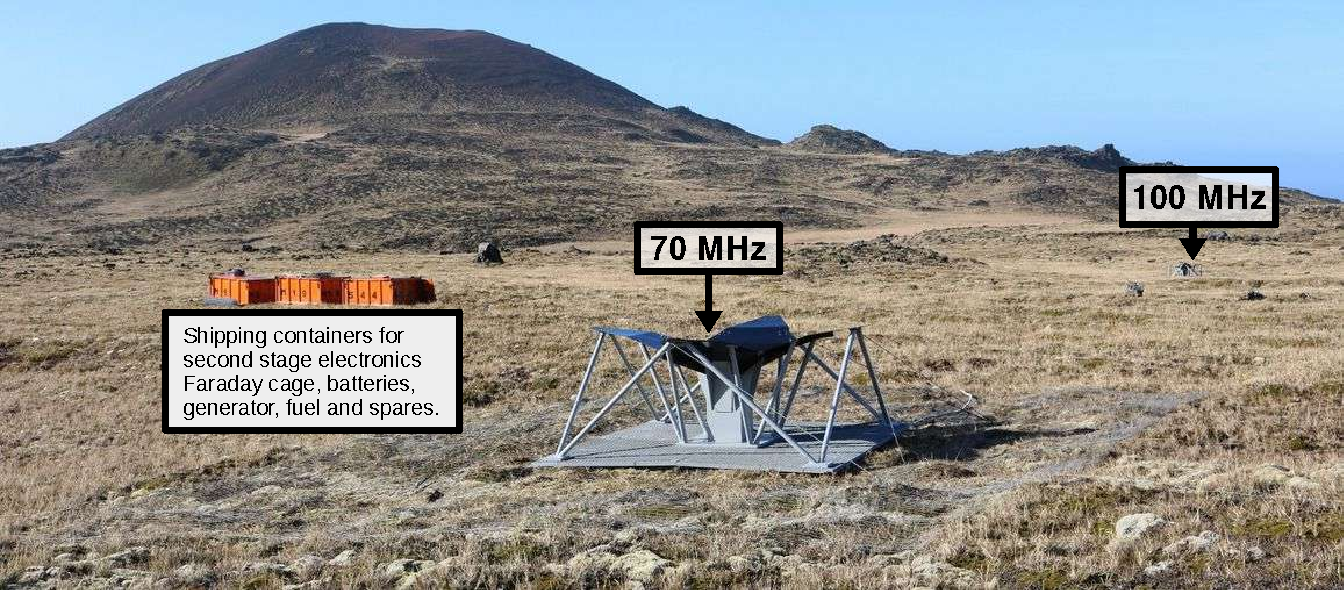
\includegraphics[width=\linewidth]{Figures/prizm.pdf}
	\caption{The \prizm\ experiment built on Marion Island. The two antennas (\SI{70}{\mega \hertz} and \SI{100}{\mega \hertz}) are visible and the the three shipping containers enclose the second stage electronics Faraday cage, generator, batteries, fuel, and spares. The main base lies four kilometers away from the observing site.}
	\label{Fig:prizm}
\end{figure}

\begin{figure}
	\centering
	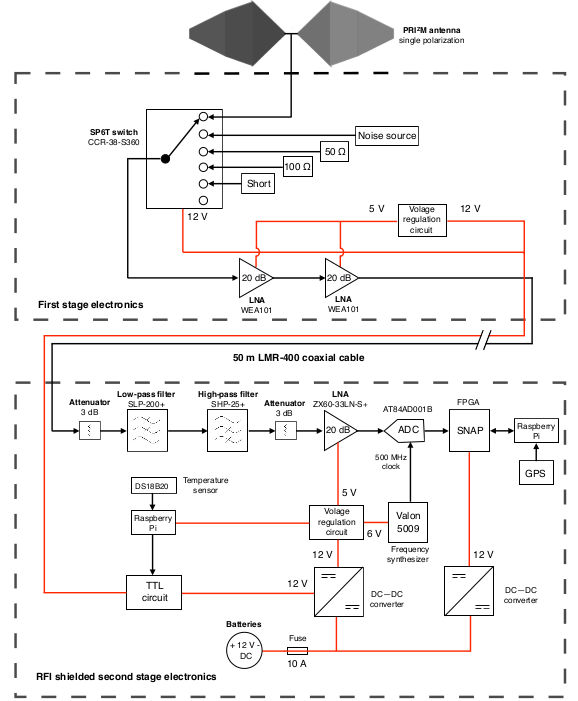
\includegraphics[width=\linewidth]{Figures/PRZIM_block}
	\caption{Block diagram for a single \prizm\ antenna polarization. The upper and lower dashed boxes \st{reflect} \attention{denote} the electronics chain's first and second stages. To decrease contamination from self-generated RFI, the 
		two stages are separated by \SI{50}{\meter}. \attention{[State figure source]}}
	\label{Fig:PRZIM_block}
\end{figure}

\section{Signal Chain}

\subsection{Antenna}

Figure~\ref{Fig:PRZIM_block} shows the \attention{original 2017 configuration of the signal chain for a} single polarization of the  \prizm\ antenna. The \st{first incarnation of the antennas, known as} \attention{antenna design was originally developed for} Sonda Cosmologica de las Islas para la deteccion de HIdrogeno neutro (SCI-HI), \attention{which} was deployed in Guadalupe Island (\SI{200}{\kilo \meter} off the coast of Mexico) in 2013. Figure~\ref{Fig:petals} shows the antenna that is made up of four petals that form a pair of crossed dipoles.

Each petal has three trapezoidal facets angled at various angles with respect to the ground to reduce the radiation pattern variations with frequency \attention{[rephrase this sentence: the angles were selected to minimize spectral variation in the beam shape]}. The antenna radiation pattern's \attention{[use ``beam'' instead of ``radiation pattern'' here and elsewhere since it's a more compact term, although you may wish to initially define the beam as the radiation pattern of the antenna]} width has a direct dependence on the angles of the trapezoidal facets, and the height of the antenna above the ground changes the beam symmetry~\citep{2014ApJ...782L...9V}.  The \prizm\ antenna structure was redesigned \attention{[add words to this sentence to make it clear that the redesign was with respect to the original SCI-HI design, as opposed to multiple design iterations within PRIZM]} using fiberglass from PVC pipe \attention{[see previous comment; ``fiberglass from PVC'' is a confusing way to phrase the change]} structure to survive the \attention{high winds on} Marion Island \st{roaring forties} as shown in Figure~\ref{Fig:structure}.  

\begin{figure}
	\centering
	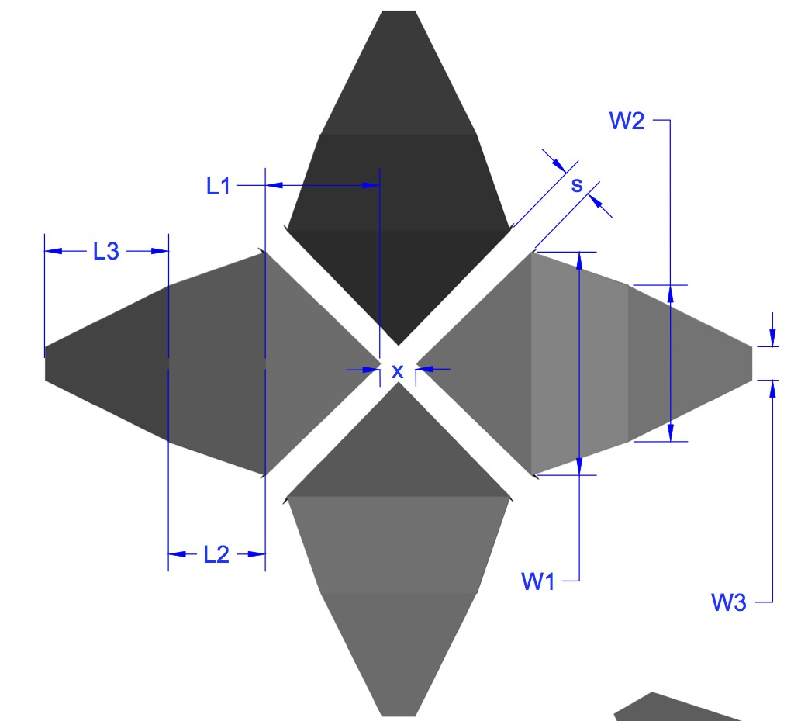
\includegraphics[width=0.7\linewidth]{Figures/petals.pdf}
	\caption{CAD picture of the \prizm\ antenna. Four-square antenna configuration which consists of two north-south and east-west aligned crossed dipoles. \attention{[I would suggest removing this figure.  The optimization of the petal geometry is described elsewhere already, and this figure isn't particularly meaningful unless you state all of the dimensions that are called out.]}}
	\label{Fig:petals}
\end{figure}

\begin{figure}
	\centering
	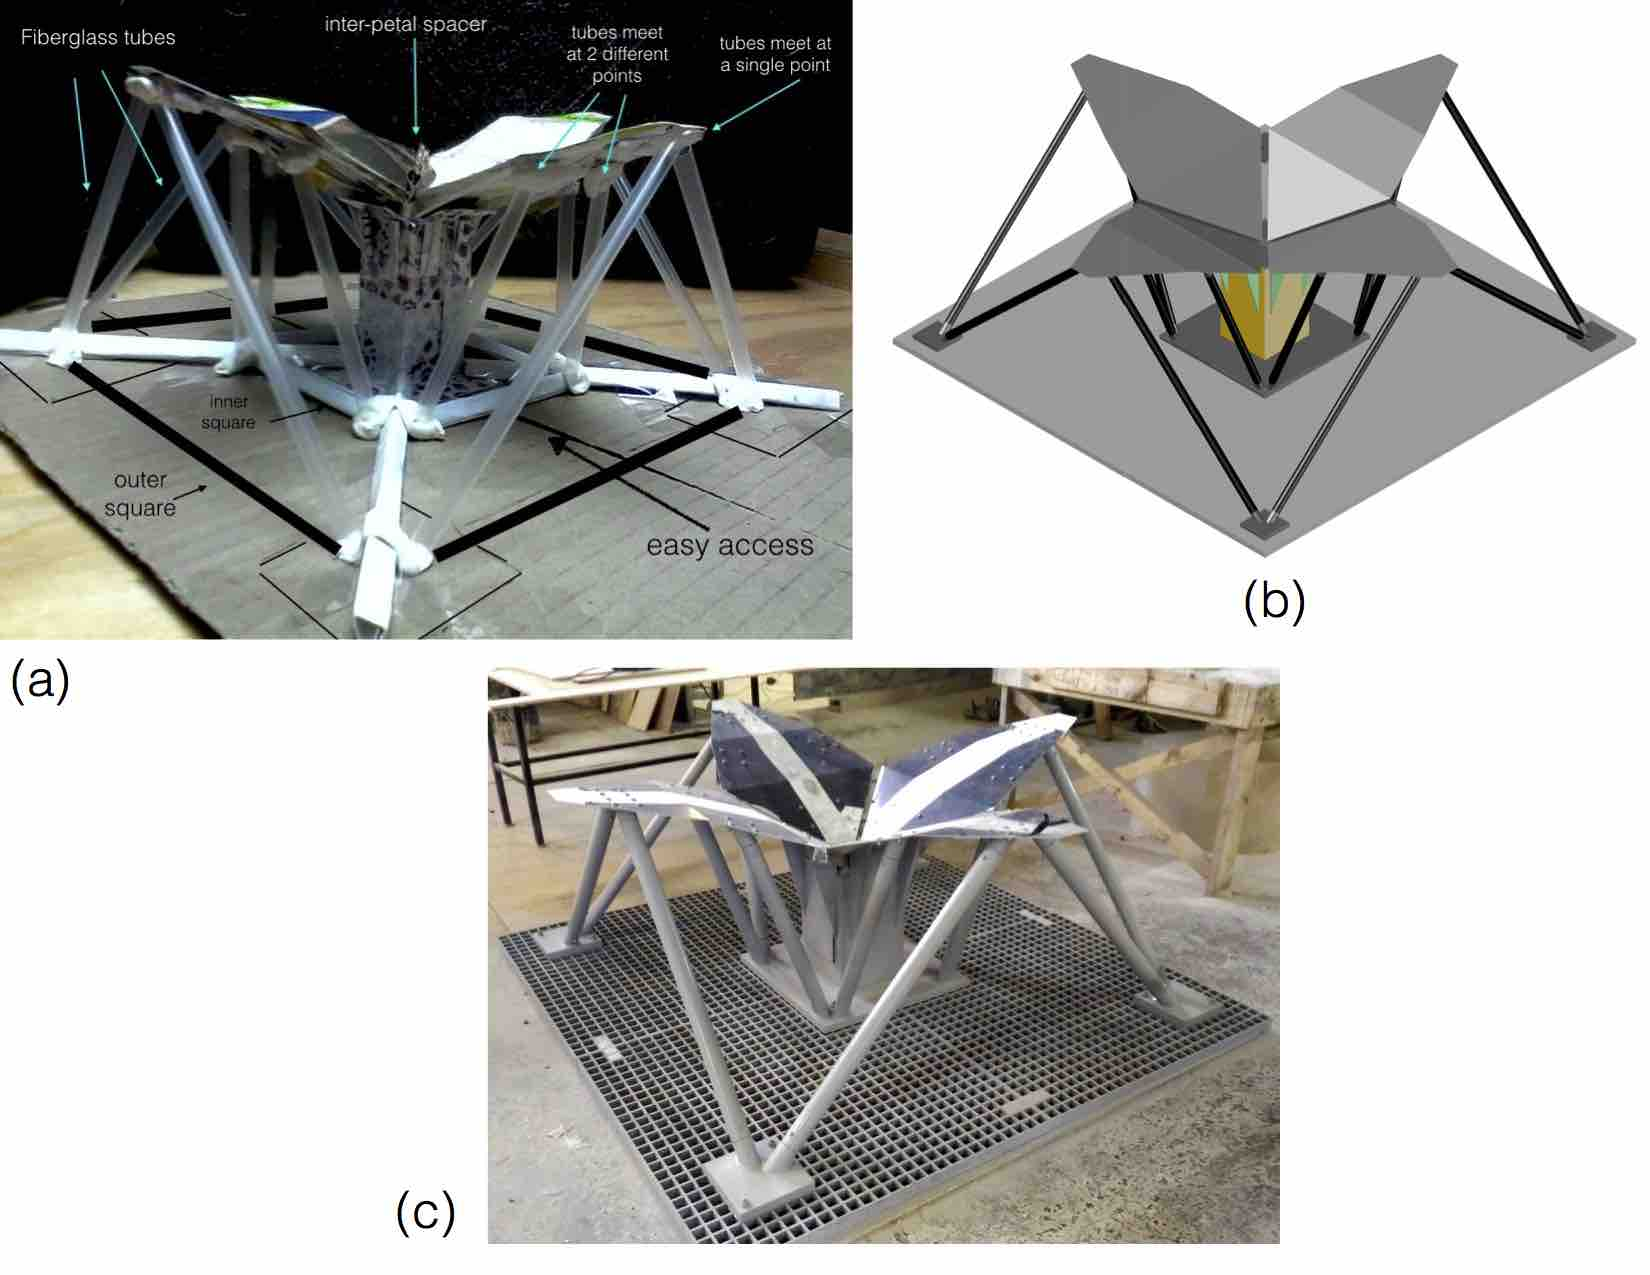
\includegraphics[width=0.7\linewidth]{Figures/structure}
	\caption{(a) A 1/10 scale model of the support structure of the \SI{100}{\mega \hertz} \prizm\ antenna made of paper and plastic straws; (b) CAD modeling; and (c) a completed \SI{100}{\mega \hertz} antenna mounted on a \SI{2x2}{\meter} fibreglass grating. \attention{[Replace this figure with a single image of the antenna operating in the field since the design work is already described in Liju's thesis.  In the caption, quote the approximate dimensions of the antenna so that the reader has a sense of scale.]}}
	\label{Fig:structure}
\end{figure}

\subsection{First Stage Electronics}

The first stage electronics \st{is} \attention{are} housed in the column supporting the antenna petals as shown in Figure~\ref{Fig:column}, and the block diagram of the first stage electronics is shown in Figure~\ref{Fig:prizm_fee_block}. The signal from \st{the} \attention{each} single-polarisation \prizm\ dipole is fed to \st{the} \attention{an} electromechanical switch \st{labeled as "calibrator switch"} \attention{[change the label in Figure 4.6 to read ``electromechanical switch'' to be consistent]} by a coaxial cable which is \SI{200}{\milli \meter} long. In order to dissipate the current on the outer conductor of the coaxial cable, a ferrite core is used. The \st{calibrator} \attention{electromechanical} switch is required to switch between observations of the sky and the calibrator sources of \SI{50}{\ohm}, \SI{100}{\ohm}, short terminators, and a broadband noise source, \attention{which are connected to the switch input terminals}. \attention{[Don't break the paragraph here.]}

\begin{figure}
	\centering
	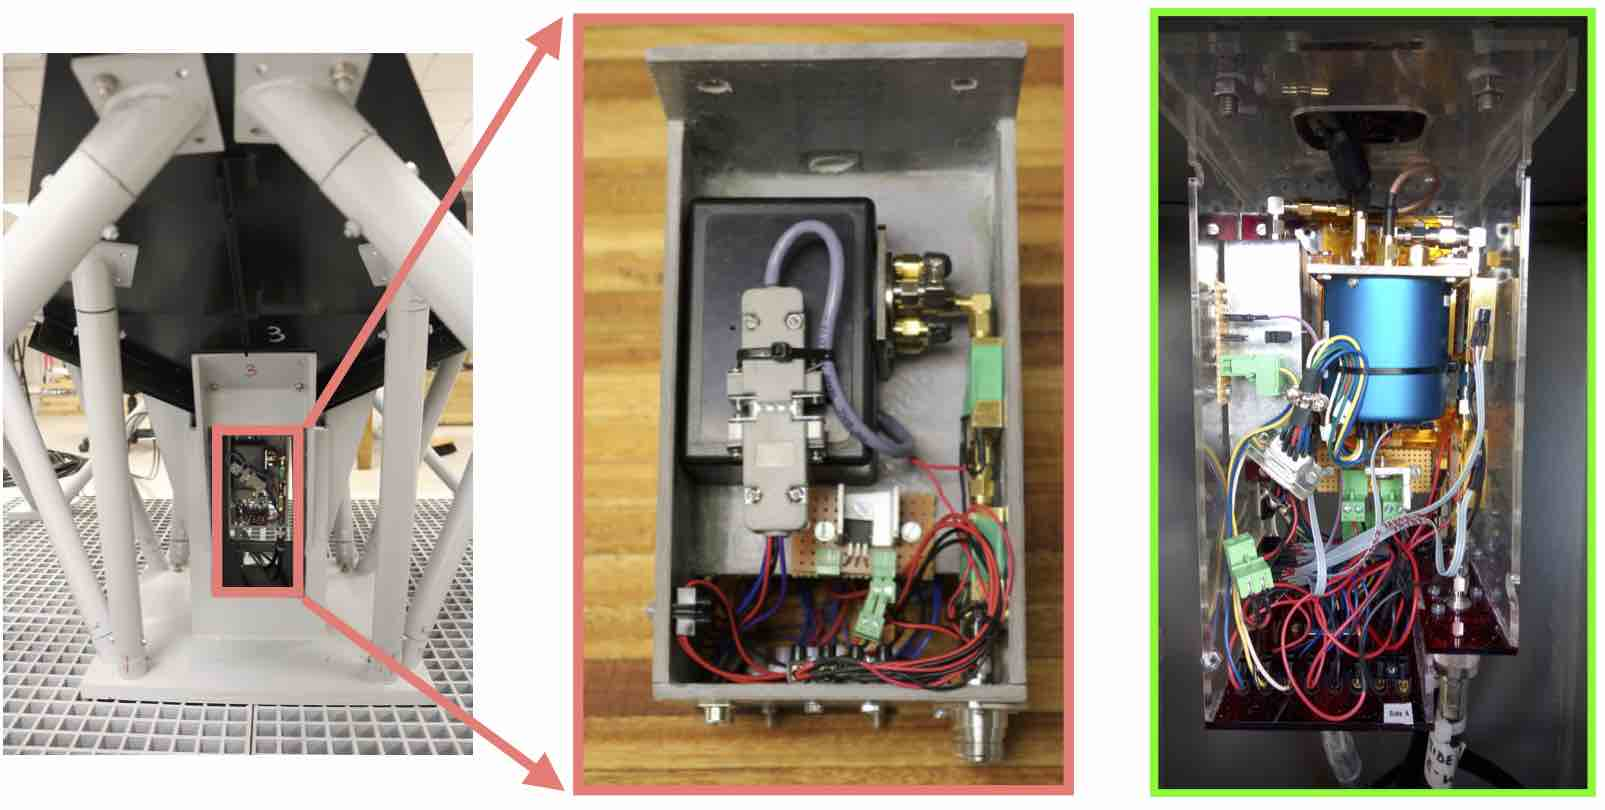
\includegraphics[width=0.7\linewidth]{Figures/column}
	\caption{The electronics box for the first stage\attention{.}\st{,}  \attention{[Break/start sentence here, state that pink was the original install from 2017, and green shows the 2018 upgrade]} green inset represents what is currently installed in the central column under the antenna.}
	\label{Fig:column}
\end{figure}

\st{Antenna and calibrator sources are connected at the calibrator switch's input ports, and the} \attention{Two cascaded} WEA101 LNAs are used to amplify \st{its} \attention{the selected signal at the switch} output. Additional electronics in the first stage electronics box include voltage regulation circuitry for LNAs and temperature sensors.  \attention{[Briefly describe the differences between the two versions of the front end that are shown in the figure (pink and green boxes).  The two major changes going from the 2017 to 2018 version are upgrading to a latching switch, adding the noise source, and distributing thermometry across the components indicated in Figure 4.6.]}

\begin{figure}
	\centering
	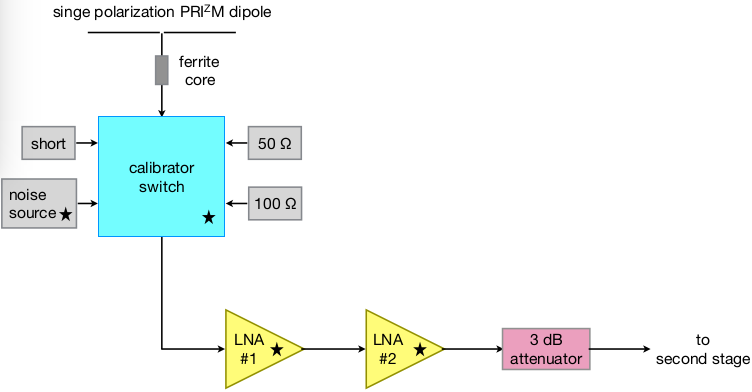
\includegraphics[width=\linewidth]{Figures/prizm_fee_block}
	\caption{A simplified schematic of electronics from the first stage. Components marked with a star are \st{connected to} \attention{outfitted with} one-wire digital temperature sensor\attention{s} \st{to record the temperature difference across them}.  \attention{[Make it clear that this diagram reflects the 2018 configuration.]}}
	\label{Fig:prizm_fee_block}
\end{figure}  

\subsection{Second Stage Electronics (SSE)}

A custom-designed Faraday cage (\SI{\sim 300x470x240}{\milli \meter} \attention{[don't nest parentheses; move the dimensions to a separate sentence later on since this information isn't important enough to put up front]} (Figure~\ref{Fig:47093285614_63bb00be20_o})) that encloses the SSE is housed in one of the shipping containers shown in Figure~\ref{Fig:prizm}. The signal from the first stage electronics is fed via a \SI{\sim 50}{\meter} LMR400 coaxial cable, which is a reasonable distance to minimize the contamination \st{of} \attention{from} possible self-generated RFI. The coaxial cables are mouse-proofed using a few meters of stainless steel wire mesh cloth \attention{wrapped near the cable penetration points}. The multi-tiered interior of the Faraday cage is shown in Figure~\ref{Fig:enclosure_ann} with the top panel removed. \attention{[Explain what you mean by multi-tiered, since the reader doesn't have a sense of the overall architecture at this point.  Give a high level description that the readout box services both antennas.  There's a separate readout chain for each antenna, but the housekeeping and switch control electronics are shared between the antennas.]}

The main power to the SSE box is fed through a BNC connector. The SSE box houses the two DC-DC converters on the bottom layer, two SNAP boards powered from one DC-DC converter, and the other DC-DC converter powers the rest of the box's electronics. \attention{[Move the power discussion to the end.  You want to organize this discussion in order of importance and signal flow, so the first thing to discuss is the second-stage RF electronics, followed by the SNAP readout.  Then housekeeping, then power.]} The filtering and amplification stage consists of the Minicircuits SLP-200+ and SHP-25+ low and high pass filters. The filtered signal is amplified by \SI{20}{\decibel} using a Minicircuits ZX60-33LN-S+ amplifier. The output signal is then fed to the readout electronics.  \attention{[Clarify that this filtering and amplification is applied to each polarization from each antenna.  Also state the gain and combined bandpass.]}

Each SNAP board receives the two RF signals from the two polarizations of a single antenna and samples the signals at a rate of \SI{500}{\mega samp\per \second} using a dual, monolithic, eight-bit, AT84AD001B external analog-to-digital converter (ADC) that is connected to the SNAP board via a Z-Dok connector. A Valon 5009 frequency synthesizer provides the ADC with a clock signal. \st{A frequency range between 0 MHz to 250 MHz containing 4096 channels is created by t}\attention{T}he SNAP board\st{, which also includes the} \attention{employs a} \st{onboard} Xilinx Kintex 7 FPGA \attention{to} \st{that} compute\st{s} auto\attention{-} and cross\attention{-}spectra from and between the four inputs\attention{, with 4096 frequency channels spanning 0--250~MHz}. An RPi controls the SNAP board and saves data to an onboard SD-card. The RPi's timing is provided by \st{the} \attention{an} Adafruit Ultimate GPS module, connected to an external \attention{active} GPS antenna.

The SSE box also encloses the additional hardware that controls the calibrator switch states and voltage regulation. The L298 full-bridge drivers were used to make the control circuit \attention{[You worked quite a bit on this circuit, right?  Include a schematic and give some more details about how it works.]}, and the transistor-transistor-logic (TTL) is used to generate the control signals. A Rpi controls the logic gates of the integrated chips. The whole first stage electronics is temperature monitored using the 1-wire DS18B20 temperature sensor \attention{[including the housekeeping schematic will help make this part of the description more clear too]}.

\begin{figure}
	\centering
	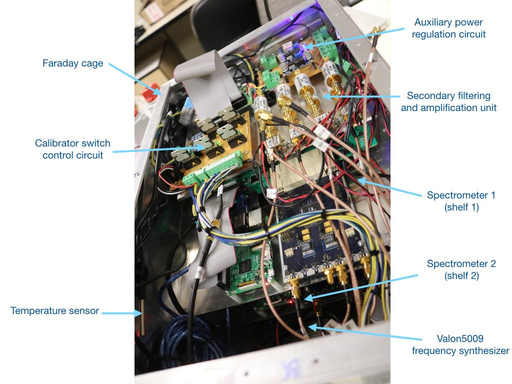
\includegraphics[width=\linewidth]{Figures/enclosure_ann}
	\caption{The multi-tiered interior shown while the SSE box top panel is removed. Most of the internal components in this configuration can be accessed, but one more panel needs to be opened to access the DC-DC converters.}
	\label{Fig:enclosure_ann}
\end{figure}

\begin{figure}
	\centering
	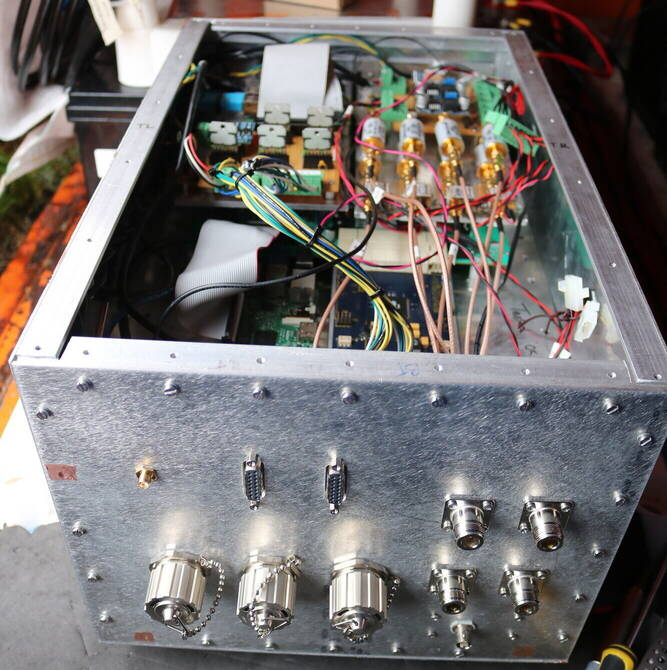
\includegraphics[width=0.4\linewidth]{Figures/47093285614_63bb00be20_o}
	\caption{The SSE Faraday cage made with separate brackets and flat sheets.}
	\label{Fig:47093285614_63bb00be20_o}
\end{figure}       

\subsection{Power}

The \prizm\ system is powered using eight \SI{12}{\volt} \SI{200}{\ampere \hour} battery bank wired in parallel as shown in Figure~\ref{Fig:power}. The total system draws \SI{\sim 65}{\watt}\st{.}\attention{, and}
\st{Moreover,} when the batteries are fully charged, the system can operate for \attention{approximately} one week. Battery charging is performed manually using a Honda EU30is generator, and a fuel cache kept at the observing site. The batteries are connected to two DC/DC converters during observations. The DC-DC converters are enclosed in the SSE box and provides stable voltage outputs despite the slow decline of the battery voltage. Further regulation is performed to supply power to several components in the system.

\begin{figure}
	\centering
	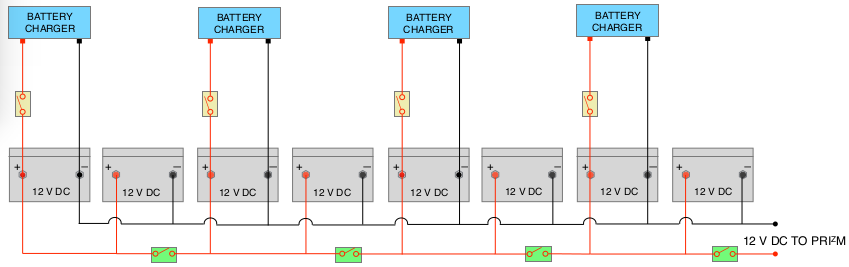
\includegraphics[width=\linewidth]{Figures/power}
	\caption{\prizm's power distribution chain consists of eight \SI{12}{\volt} \SI{200}{\ampere \hour} lead crystal batteries each. The batteries work in pairs that, through the green switches, are cascaded together. The battery pairs are disconnected during charging, and a single battery charger \st{will} charge\attention{s} two batteries \attention{simultaneously}. To \st{power} \attention{connect} the battery chargers, yellow switches are used. All yellow switches are turned OFF during the observation, and all green switches are powered ON.}
	\label{Fig:power}
\end{figure}

\section{Revised \prizm~Instrumentation}

\attention{This section describes} revisions \attention{that} were \st{done} \attention{made} to some of the \prizm\ subsystems \attention{in preparation for the 2020 voyage to improve functionality and performance} \st{as part of maintenance and functionality improvement}. The \st{proposed} \attention{redesign of the} first stage electronics enclosure \st{design} will be discussed in the next subsections, together with the revised SSE enclosure. \st{The rest of the electronic parts and subsystems are going to remain the same.} Due to COVID-19 restrictions, \attention{the redesigned first stage electronics and SSE were not fully integrated and tested, and this section reports the work that was completed before lockdowns began.} \st{the proposed first stage electronics and their enclosure were not assembled, tested, and implemented, nor the SSE enclosure.}  \attention{[You can add a footnote stating that the 2020 voyage was cancelled because of COVID-19.]}

\subsection{First Stage Electronics (FSE)}

\st{After assessing the current FSE and its functionality, a} \attention{A} new FSE and \st{its} enclosure were proposed for \st{an upcoming} \attention{the 2020} deployment. Figure~\ref{Fig:FSE_rev} shows the block diagram of the proposed FSE architecture. \attention{[Include a high level description explaining what the major changes were and the motivations for those changes.]} To ensure that the enclosure was going to hold all the FSE, dummy placeholder components were crafted and placed in the enclosures. Figure~\ref{Fig:FSE_archi} shows a nominal component layout with dummy placeholders. Enclosures are two off-the-shelf boxes that are attached back to back for the two polarizations. Most of the housekeeping electronics are on the side of Figure~\ref{Fig:FSE_archi}, which is intended to be accessed from the east-facing column door, giving the human slight shelter from the \attention{prevailing} wind. The only housekeeping breakout on the second enclosure is half of the one-wire thermometry bus.

\begin{figure}
	\centering
	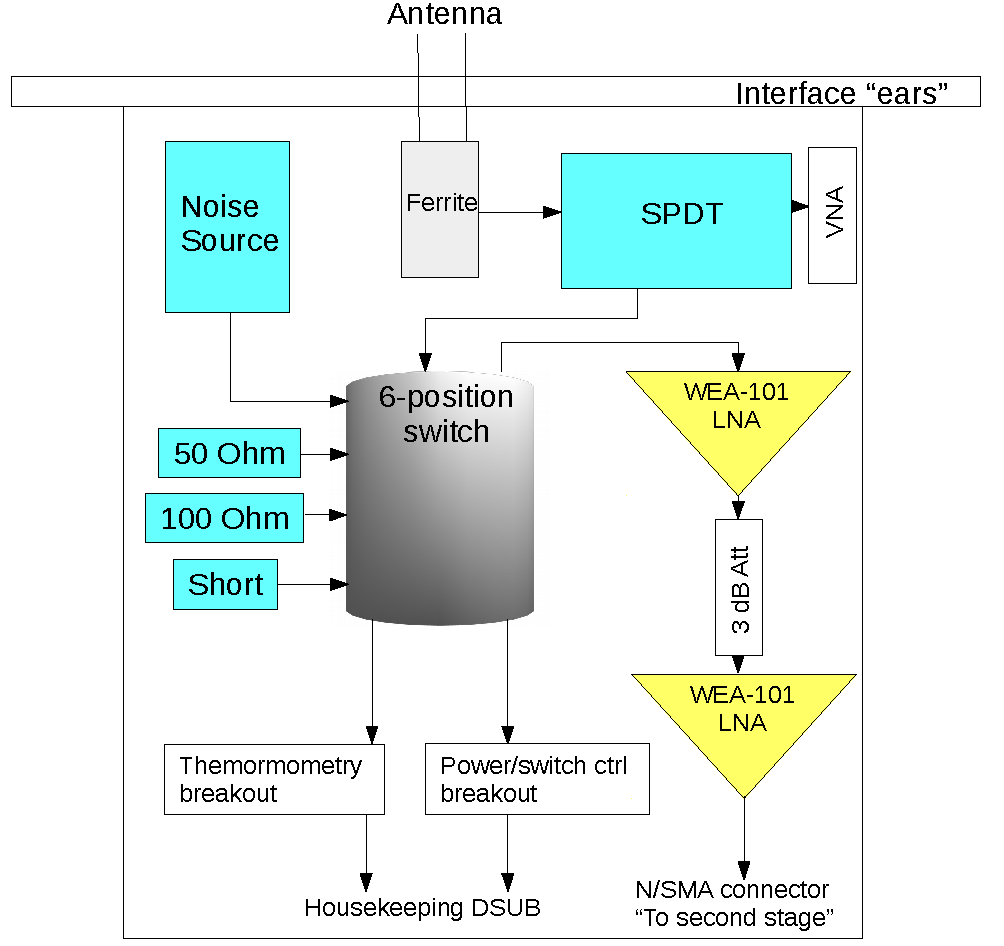
\includegraphics[width=0.7\linewidth]{Figures/FSE_rev}
	\caption{The block diagram of the proposed FSE achirtecture showing the 6-position switch connections, the breakouts for housekeeping, SPDT for controling the SP6T and amplification. \attention{[Remove the arrow between the SP6T and thermometry breakout, since that connection would imply that switch signals are being passed to the thermometers.  Clarify in the caption that the VNA isn't permanently installed, and the box you've drawn indicates a connection point.]}}
	\label{Fig:FSE_rev}
\end{figure} 

The box currently accommodates only one SPDT switch per side instead of two. \attention{[This is a brand new addition.  Your text should introduce the addition of the new SPDT switch, and explain that we're considering adding others in the future.  In all cases, explain the reasoning and motivation.]} The SPDT switch helps us to look through the antenna without any cables being physically disconnected.  \attention{[Explain the previous sentence in more detail.  For example, describe how VNA calibration is performed with the existing system, and specify which cables need to be disconnected for the procedure.  Then describe exactly how the SPDT switch solves this problem.]}  A right-angle adapter will be required on the SPDT to interface with the Y-cable. To look into the 6-position switch \attention{[be more specific: instead of saying ``look into,'' state which S parameters are useful to measure and where the connections have to be made]}, a VNA will be plugged directly into an open port for the time being. The terminal blocks have 16 positions total, so one is unused by the DB-15 breakout\st{. T}\attention{ (and t}he SP6T switch can block the unused position\attention{)}. The filters in Figure~\ref{Fig:FSE_archi} are placeholders, but they are about the same size as the WEA-101 LNAs highlighted in yellow in Figure~\ref{Fig:FSE_rev}. In Figure~\ref{Fig:FSE_archi}, the incoming DB-15 connector is split out into two terminal blocks, and Table~\ref{Tab:Pinout} shows the connection configuration. The wall-mounted PCB has a 12V input and provides the LNAs with a 5V output and the one-wire thermometers with a 3.3V onboard output. To service both polarizations, all one-wire thermometers are connected to the three-row header, which is split into two parts \attention{[be more clear here: all thermometers servicing both polarizations are ganged together on a single bus, so the headers are split accordingly across the two halves of the enclosure]}.

\attention{Other things you can mention in this section are that we're
  using off the shelf enclosures rather than custom geometries, and
  the new boxes give us slightly more room (to house the SPDT switch).
  The perforated gray sheet serves as a mechanical breadboard for easy
  addition of new parts without having to drill the enclosures
  themselves.}

\begin{figure}
	\centering
	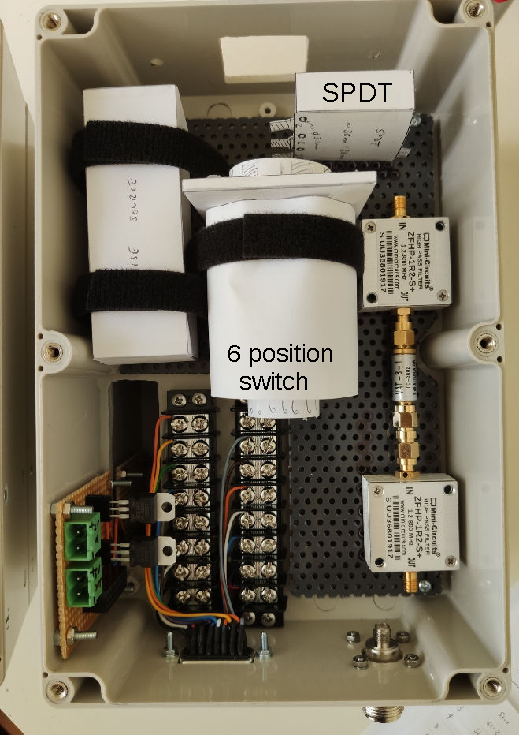
\includegraphics[width=0.5\linewidth]{Figures/FSE_archi}
	\caption{General layout of the components in the proposed FSE enclosure with dummy placeholders.}
	\label{Fig:FSE_archi}
\end{figure}

\begin{figure}
	\centering
	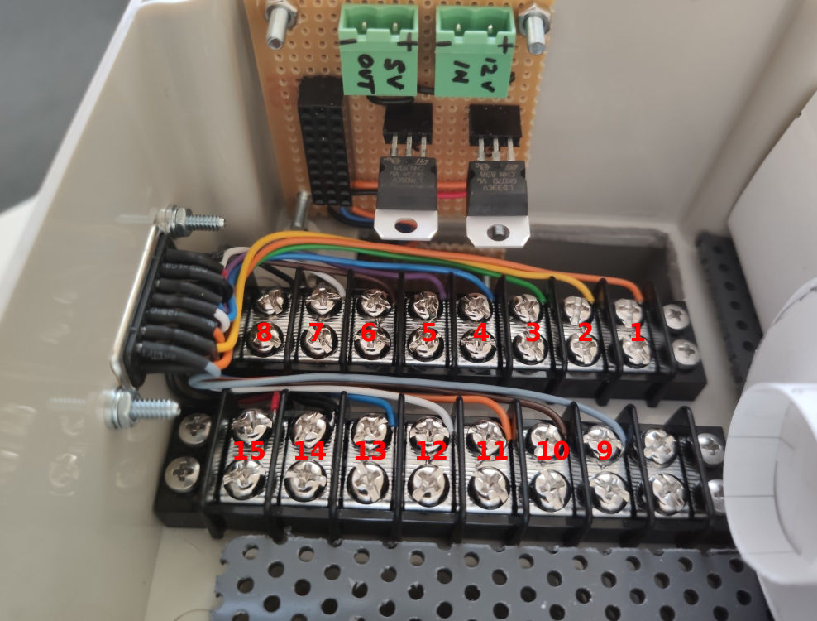
\includegraphics[width=0.7\linewidth]{Figures/Terminal}
	\caption{Housekeeping breakout. DB-15 pin assignments are annotated on the terminal blocks.}
	\label{Fig:Terminal}
\end{figure}

\begin{table}
	\centering
	\begin{tabular}{ c|c|c|c} 
		\hline
		DB-15 & Terminal Block & Colour & Function \\
		\hline
		\hline
		1 & L1 & Orange & S1-1 \\ 
		2 & L2 & Yellow & S1-2 \\ 
		3 & L3 & Green & S1-3 \\
		4 & L4 & Blue & S1-4 \\
		5 & L5 & Purple & S1-5 \\
		6 & L6 & Brown & S1-6 \\
		7 & L7 & White & S1-Reset \\
		8 & L8 & Black & Ground \\
		9 & R2 & Gray & S2-Ant \\
		10 & R3 & Brown & S2-Cal \\
		11 & R4 & Orange & Noise \\
		12 & R5 & White & Blank \\
		13 & R6 & Blue & Temp Sensor \\
		14 & R7 & Black & Ground \\
		15 & R8 & Red & 12 V \\
		\hline
	\end{tabular}
	\caption{Housekeeping pinout. Terminal block notation and numbering L and R denote left and right as viewed when the box is vertical, and numbers are from top to bottom. S1 denotes SP6T switch, S2 denotes SPDT switch.}
	\label{Tab:Pinout}
\end{table}


\subsection{Second Stage Electronics}

A revised Faraday cage (\SI{\sim 400x280x110}{\milli \meter}) \attention{[move the size information later in the paragraph, and compare it against the dimensions of the original box]} for the SSE was designed using Autodesk Inventor Professional 2018, and the sheet metal box is shown in Figure~\ref{Fig:Enclosed}. The enclosure was revised so that each antenna has its SSE box.  There was no longer shared housekeeping RPi that binds the SNAP boards together \attention{[this is another system change that you helped with, so spend a little more time explaining the new switch circuit and include a schematic]}. That was the main driver for separating the SNAP boards/ enclosures.  

The main improvements to the new enclosure are listed below.

\begin{itemize}
	\item Increased and improved accessibility of all components, \attention{[Expand this a bit more.  Because each enclosure now services only one antenna, all components can be accommodated on a single shelf that can be accessed from both sides.]}
	\item The design is folded laser cut sheet metal, unlike the separate brackets and flat sheets that make up the current design
	\item Easier and cheaper to assemble and manufacture
	\item User-friendly (the holes are already in place to tap and screw the components in place \attention{[you can also mention the captive quarter-turn fasteners, which are a godsend for field work]})
	\item It was designed to fit into a hiking backpack for easy carrying when hiking to the \prizm\ site. \attention{[make a note that the current enclosure, servicing both antennas, is too large to conveniently carry on foot]}
	\item The new enclosure has a partitioned portion to accommodate the \attention{second stage} RF \attention{electronics} \st{signal} and ensure \attention{isolation from} \st{that} self-generated RFI \attention{from switching electronics elsewhere in the enclosure} \st{does not contaminate the RF signal}, as shown in Figure~\ref{Fig:farap}.
	\item A \st{SNAP board} cooling fan was \st{also} added \st{for stable functionality} \attention{to prevent thermal shutdowns} of the SNAP board.
	\item The switch control circuit was revised, and it is a stackable layout so that it sits on top of the RPi and connects directly to the GPIO pins.
        \item \attention{[Add a bullet here about the RF absorber sheets that you planned on adding to the lids.]}
\end{itemize}

\attention{Add a paragraph or table listing all of the components that
  are housed in this new enclosure.  Also describe the connectors on
  the front panel.}

\attention{This section ends very abruptly.  Tie it off with a short
  paragraph explaining that you got the boxes fabricated, the parts
  fit together as designed, you finished (?) installing the
  components...etc, wherever your work left off before COVID hit.}

\begin{figure}
	\centering
	\begin{subfigure}[t]{0.52\textwidth}
		\centering
		\includegraphics[width=\linewidth]{"Figures/Top Open"} 
		\caption{} \label{Fig:Top Open}
	\end{subfigure}
	\hfill
	\begin{subfigure}[t]{0.46\textwidth}
		\centering
		\includegraphics[width=\linewidth]{"Figures/Bottom Open"}
		\caption{} \label{Fig:Bottom Open}
	\end{subfigure}
	\caption{{\bf (a)} CAD of an enclosure with the top lid open. The partioned portion is to avoid self-generated contamination from components with switching mechanisms. Some placeholders were mounted on the sheet metal design on Autodesk Inventor. {\bf (b)} The bottom view without the lid, showing the SNAP board and its cooling fan, and the RPi. \attention{[Make these figures bigger, like the full width of the page!  This is your work, so you should show it off! :-)]}} \label{Fig:farap}
\end{figure}


\begin{figure}
	\centering
	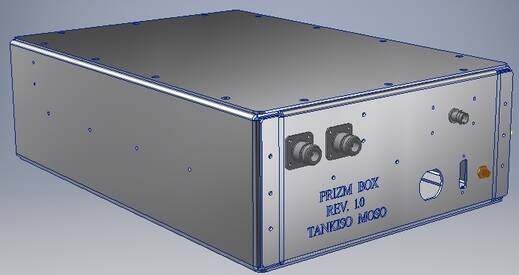
\includegraphics[width=0.7\linewidth]{Figures/Enclosed}
	\caption{An enclosed box showing the connector placeholders and measured cutouts for other connectors that are not \st{mounted} \attention{shown in this rendering}.  \attention{[Make this figure bigger, like the full width of the page!  This is your work, so you should show it off! :-)]}}
	\label{Fig:Enclosed}
\end{figure}
